\documentclass{article}

\usepackage[utf8]{inputenc}
\usepackage{amsfonts}
\usepackage{todonotes}
\usepackage{cryptocode}
\usepackage{algorithm,algorithmic}

\newcommand{\adv}{{\sf Adv}}
\newcommand{\madv}{\mathsf{Adv}}

\title{Encrypted SNI}
\author{No Name}
\date{\today}

\begin{document}

\maketitle

\section{Introduction}

In this note we try formalize the privacy goals of Encrypted SNI \cite{ietf-tls-esni-04}.

\section{Notation}

TLS is an authenticated key exchange protocol composed of sub-protocols. Importantly, TLS has
a handshake and record protocol. The handshake protocol uses handshake messages to perform
key exchange and its many facets, including, among other things, cryptographic algorithm
selection and peer authentication. Let $h \in \{0,1\}^{2^{16}}$ be a handshake message 
composed of arbitrary data, and let $\mathbf{H}$ be the set of possible handshake messages.

The record protocol uses messages with headers consisting 
of type, length, and version to send data between peers. This data is either a plaintext 
handshake message or encrypted blob. For our analysis, let $r = (d, p)$ be a 
record composed of direction $d \in \{0,1\}$ and payload $p \in \{0,1\}^{2^{16}}$. Let
$\mathbf{R}$ be the set of all possible records. Let $\mathbf{P} = \{0,1\}^{2^{16}}$ 
be the set of possible payloads. Note, by definition $\mathbf{H} \subset \mathbf{P}$.
Let $\mathsf{Message}$ be a function that returns the plaintext message for a given
record $r$, or nothing if the record is encrypted.

We model a TLS handshake as a trace of records and their metadata sent between a client and server. 
(Metadata may include, among other things, record lengths as observed on the wire.) 
Formally, let $\vec{t} = <r_0, r_1, \dots, r_n\>$ be a trace of $n$ records, where 
$r_i = (d_i, p_i) \in \mathbf{R}$. Let $\mathbf{T}$ be a set of traces. 

Without loss of generality, in TLS 1.3, there are three types of messages observed
on the wire: ClientHello (CH), ServerHello (SH), and ApplicationData (AD). Let $\mathbf{CH}$ 
and $\mathbf{SH}$ be the set of possible CH and SH handshake messages generated by 
clients and servers, respectively. Each CH, SH, and AD message belongs to $\mathbf{P}$.

Let $N \in \{0,1\}^{2^{16} - 1}$ be a name, and let $\mathbf{N}$ be the set of names. 
CH messages typically carry names as one of their parameters.

Let $\mathsf{ClientConfig}$ be a set of parameters that determine a client's configuration,
including supported ciphersuites, named groups, extensions, etc. 
Let $\mathbf{CC}$ be the set of all client configuration parameters.
Similarly, let $\mathsf{ServerConfig}$ be a set of parameters that determine a server's configuration,
and let $\mathbf{SC}$ be the set of all client configuration parameters.
Clients produce CH messages to a given server, identified by its name $N$, and configuration
$\mathsf{ClientConfig}$, using a function $\mathsf{GenerateCH}: \mathbf{N} \times \mathbf{CC}$.
Servers produce SH messages (and do other parameter selection) based on a CH message and 
server configuration, using a function $\mathsf{GenerateSH}: \mathbf{CH} \times \mathbf{SC}$.

The function $\mathsf{Metadata}$ takes as input a CH or SH and returns the set of metadata,
or parameters, associated with the message, including the server name $N$, ciphersuite list,
named groups, and other extensions that are visible on the wire. The function
$\mathsf{PublicMetadata}$ returns the same output as $\mathsf{Metadata}$, except that
the server name is omitted. 

Using the notation above, every handshake is a probabilistic function of some server name $N$,
$\mathsf{ClientConfig}$, and $\mathsf{ServerConfig}$. In particular:
%
\begin{itemize}
    \item A client generates a CH message using $N$ and $\mathsf{ClientConfig}$.
    \item The recipient server generates a SH message using the input CH and $\mathsf{ServerConfig}$.
    \item The remainder of the handshake contains encrypted AD messages.
\end{itemize}
%
Thus, let $\mathsf{Handshake}$ be a function that takes as input $N$,
$cc = \mathsf{ClientConfig}$, and $sc = \mathsf{ServerConfig}$ and produces a trace 
$t = r_1, r_2, r_3, \dots$, where $\mathsf{Message}(r_1)$ is a CH and 
$\mathsf{Message}(r_2)$ is a SH. Let $\mathsf{PublicHandshake}$ be a similar
function that computes $t = r_1, r_2, r_3, \dots = \mathsf{Handshake}(t, cc, sc)$ and returns 
$t^v = \mathsf{PublicMetadata}(r_1), \mathsf{PublicMetadata}(r_2), r_3, \dots$. That is,
it returns publicly visible metadata associated from a handshake trace. 

Finally, we define a function $\mathsf{SNI}$ which takes as input a handshake trace $t$
and returns the name $N$ which was used to generate $t$. 

\section{Security Model}

In this section, we describe two variants of an ESNI adversary: passive and active. We derive 
definitions from the classic "find-and-choose" notion of indistinguishability. Informally, 
in each game, the adversary \adv\ is given information about a game and must present two options
for the challenger. The challenger chooses one option at random and presents the result of some 
operation applied to the selected option to \adv, who must then identify which of 
the two options was selected. (This is typically the encryption of one message.) If the 
\adv's advantage in making this selection is negligibly later than $0.5$, then the options 
are indistinguishable under the challenger's operation.

In porting this definition to ESNI, we seek to capture indistinguishability of handshake traces
derived from names. That is, the challenger's operation is to generate a public handshake trace 
based on a randomly chosen name. Specifically, \adv\ chooses two names $N_0$ and $N_1$ during
a ``find'' phase, and presents them to the challenger $C$. $C$ then generates 
$t_b^v = \mathsf{PublicHandshake}(N_b)$, where $b \gets \{0,1\}$, and presents this to \adv. 
The adversary then presents its selection $b'$ to the challenger. The output of the game
depends on whether or not $b = b'$. This is shown in Figure \ref{fig:passive-game}.

\begin{figure}
    \centering
    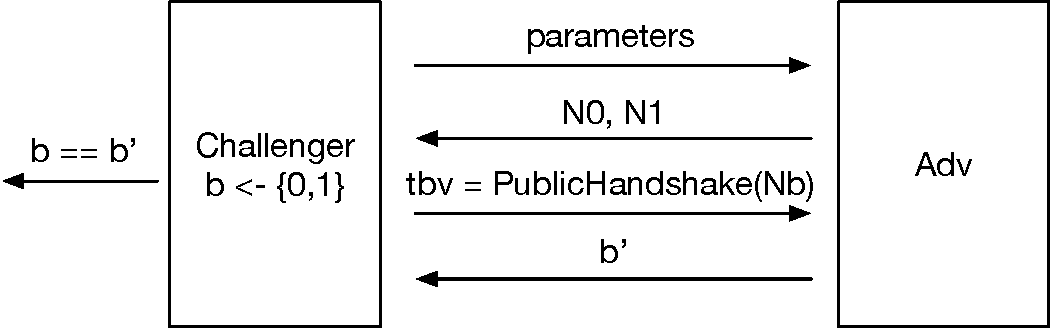
\includegraphics[scale=0.7]{esni_game.pdf}
    \caption{Passive ESNI Privacy game}
    \label{fig:passive-game}
\end{figure}

We capture this definition in the following {\sf NameGame}, which is defined in Algorithm \ref{alg:esnigame}.

\begin{algorithm}
\caption{{\sf NameGame}} 
\label{alg:esnigame}
\begin{algorithmic}[1]
  \STATE On input security parameter $\lambda$, $\mathbf{N}$, $\mathbf{CC}$, $\mathbf{SC}$, and adversary \adv\, a challenger $C$ initializes \adv\ with $\mathbf{CC}$, $\mathbf{SC}$, and $\mathsf{N}$. 
  \STATE \adv\ presents the challenger with two distinct names $N_0$ and $N_1$, where $N_0 \not= N_1$.
  \STATE $C$ chooses a random bit $b$ and returns $t_b^v = \mathsf{PublicHandshake}(N_b)$ to \adv.
  \STATE \adv\ replies with a bit $b'$.
  \STATE Output $1$ if $b = b'$, otherwise output $0$.
\end{algorithmic}
\end{algorithm}

We say that \adv\ wins $\mathsf{NameGame}$ if it outputs $1$, i.e., if \adv\ was able to determine distinguish 
two handshakes using the same ESNI (or not). We define the advantage \adv\ has in this game as
$|\Pr[\mathsf{NameGame}(\lambda, \mathbf{N}, \mathbf{CC}, \mathbf{SC}, \madv)] - \frac{1}{2}|$. That is, 
the probability that \adv\ guesses $b$ correctly less the probability that it guesses incorrectly. 

We say that a handshake trace is \emph{SNI agnostic} if, for all PPT adversaries \adv, \adv's advantage in 
winning $\mathsf{NameGame}$ is negligibly small in $\lambda$. 

\subsection{Active Adversary}

An active adversary has the ability to generate handshake traces at will. We assume servers are neither malicious nor compromised. 
Therefore, adapting our model for privacy requires extending $\mathsf{NameGame}$ to give \adv\ an oracle for producing handshake
traces with an SNI of its choosing. We define this oracle as $\mathcal{O}_H$, and it takes as input an SNI $N \in \mathbf{N}$
and returns a handshake trace $H(N) \in \mathbf{H}$. The modified game, called $\mathsf{ActiveNameGame}$, proceeds as follows:

\begin{algorithm}
\caption{{\sf ActiveNameGame}} 
\label{alg:active-esnigame}
\begin{algorithmic}[1]
%   \scriptsize
  \STATE On input security parameter $\lambda$, $\mathbf{N}$, $\mathbf{CC}$, $\mathbf{SC}$, and adversary \adv\, a challenger $C$ initializes \adv\ with $\mathbf{CC}$, $\mathbf{SC}$, $\mathsf{N}$, and access to $\mathcal{O}_H$.
  \STATE \adv\ queries $\mathcal{O}_H$ with names values of its choosing from $\mathbf{N}$ at most $\mathsf{poly}(\lambda)$ times.
  \STATE \adv\ presents the challenger with two distinct names $N_0$ and $N_1$, where $N_0 \not= N_1$.
  \STATE $C$ chooses a random bit $b$ and returns $t_b^v = \mathsf{PublicHandshake}(N_b)$ to \adv.
  \STATE \adv\ continues querying $\mathcal{O}_H$ at most $\mathsf{poly}(\lambda)$ times.
  \STATE \adv\ replies with a bit $b'$.
  \STATE Output $1$ if $b = b'$, otherwise output $0$.
\end{algorithmic}
\end{algorithm}

As before, we say that \adv\ wins $\mathsf{ActiveESNIGame}$ if it outputs $1$. 
We define the advantage \adv\ has in this game as
$|\Pr[\mathsf{ActiveESNIGame}(\lambda, \mathbf{N}, \mathsf{config}, \madv)] - \frac{1}{2}|$. And we say that a handshake trace
is \emph{SNI agnostic} with respect to an active attacker if \adv's advantage in winning $\mathsf{ActiveESNIGame}$ is negligibly 
small in $\lambda$.

\bibliographystyle{plain}
\bibliography{references}

\end{document}
